\documentclass[10pt, a4paper]{article}
\usepackage[T1]{fontenc}
\usepackage[utf8x]{inputenc}
\usepackage{ifpdf}
\usepackage{graphicx}
\usepackage{array}
\usepackage{multirow}


\usepackage{listings}	% For program listings.
\usepackage{color}
\definecolor{dkgreen}{rgb}{0,0.6,0}
\definecolor{gray}{rgb}{0.5,0.5,0.5}
\definecolor{mauve}{rgb}{0.58,0,0.82}
\lstset {
	language=Matlab,			  		% The language of the code.
	basicstyle=\footnotesize,			% The size of the fonts that are used for the code.
	numbers=left,						% Where to put the line-numbers.
	numberstyle=\tiny\color{gray},		% The style that is used for the line-numbers.
	stepnumber=1,						% The step between two line-numbers. If it's 1, each line will be numbered.
	numbersep=5pt,						% How far the line-numbers are from the code.
	backgroundcolor=\color{white},		% Choose the background color. You must add \usepackage{color}.
	showspaces=false,					% Show spaces adding particular underscores.
	showstringspaces=false,				% Underline spaces within strings.
	showtabs=false,						% Show tabs within strings adding particular underscores.
	frame=single,						% Adds a frame around the code.
	rulecolor=\color{black},			% If not set, the frame-color may be changed on line-breaks within not-black text (e.g. comments (green here)).
	tabsize=2,							% Sets default tabsize to 2 spaces.
	captionpos=t,						% Sets the caption-position to bottom.
	breaklines=true,					% Sets automatic line breaking.
	breakatwhitespace=false,			% Sets if automatic breaks should only happen at whitespace.
	title=\lstname,						% Show the filename of files included with \lstinputlisting;  also try caption instead of title.
	keywordstyle=\color{blue},			% Keyword style.
	commentstyle=\color{dkgreen},		% Comment style.
	stringstyle=\color{mauve},		  	% String literal style.
	escapeinside={\%*}{*)},			  	% If you want to add a comment within your code.
	morekeywords={*,...}			  	% If you want to add more keywords to the set.
}

\newcommand{\matlab}{\small{\emph{MATLAB\textsuperscript{\textregistered}}}}
\newcommand{\excel}{\emph{Microsoft Excel\textsuperscript{\textregistered}}}

\title{Numerical Analysis for Computer Scientists\\ FMN011, Lund University 2012\\ Project \#2\\ Finding the line strength of stars for an astronomer}
\date{}
\author{Erik Westrup, \texttt{<ada09ewe@student.lu.se>}}

\begin{document}
\begin{titlepage}
\maketitle

\thispagestyle{empty}
\end{titlepage}
\setcounter{page}{2}

\section{Introduction and Problem Background}
This project is about solving real-world problems with their accompanied complexities and ambiguities. The best method must be determined and its limitations and possible errors must be known. In this project intensity of light from stars will be studied. Stars produces a continuous curve of light over a range of frequencies called the \emph{spectrum} for that star. It can be measured in \emph{relative intensity} ($\frac{\mathrm{W}}{\mathrm{m}^2\times\mathrm{Hz}}$) as a function of the frequency (Hz) which is defined as the spectrum. We want to measure in relative intensity because  the energy is higher at higher frequencies and that known property is not the one we want to study. Therefore we normalize it with the frequency. 

What is interesting is that the surrounding gases of a star will either absorb (cold gas) or emit (warm) light which is visible at discrete fixed frequencies in the spectrum as \emph{spectral lines}. By identifying these spectral lines the components of the star can be found  because each chemical composition have a unique fingerprint of discrete frequencies \cite{astronotes1} \cite{astronotes2}.

In this project a measured continuous spectrum for a star is given which contains six spectral lines evenly divided in absorption lines and emissions lines. The task is to find the total intensity for each of these spectral lines called the \emph{line strength} measured in $\frac{\mathrm{M}}{\mathrm{m}^2}$ \cite{linestrength}. This is achieved by finding the area under the curve at the peak-frequencies i.e. integrating the relative intensity over these frequencies. % TODO why do you want the area?

The areas can not be found using analytical methods since we don't have the real spectrum and spectrum line functions -- just observations from it. We must find a way of finding the area from just these observations.

The given data is a file with $4000$ measurements of \emph{Specific Intensity} in $\frac{\mathrm{W}}{\mathrm{m}^2\times \mathrm{Hz}}$ at frequencies in the range $[3.50\times10^{14}, 4.29\times10^{14}]$.

\section{Numerical Considerations}
For this problem there was no hints on what methods to be used. Therefore an iterative approach was used to find methods that works. The process will be describe in section \ref{sec:result}. As described there, I used some \matlab features including polynomial fitting in the least squares sense with the command \emph{polyfit} and estimation of areas using the trapezoidal method with the command \emph{trapz}. As later described there was a problem with an ill-conditioned matrix which was solved my normalization.

\section{Results \& Analysis} \label{sec:result}
All code used to get the results can be seen in Appendix \ref{appendix:programs}. The first thing to do is, as always, to get an understanding of what are the given. Since studying the raw data is hard a graphical plot over the curve is desired to grasp the main characteristics of what we have. The relative intensity spectrum can be seen in figure \ref{fig:rellspec} and the spectrum itself in figure \ref{fig:spec}. In these two plots the six spectral lines are clearly visible. Just because it is interesting, the intensities are also show as a function of the wave lengths in figure \ref{fig:specwave} using the \matlab function \emph{spectrumLabel}\cite{spectrumLabel}.

The first na\"{i}ve thing to do is to see if we can fit a curve the data directly. Just by trying out some, one seen in figure \ref{fig:badfit}, we can conclude that no polynomial can fit both the spectrum and the spectrum lines and give a good representation of the real functions. From this the main idea for solving this project was developed. We want to find a function representing the spectrum and then approximate the area between this function and the peaks/dips.

To find this function we must first remove the distracting points from the spectrum lines and extrapolate the missing parts of the spectrum line. By plotting the data points as a function of their index in a graph the beginning, midpoints and endpoints for peaks/dips could be found. One had to zoom in very much in the graph to really see the hidden details of the slope. From these points some polynomial fittings was done as seen in figure \ref{fig:goodfit}. This of course depends on eye measurements which is not exact so I made sure to have some small marginals by removing possibly more points than needed. This is not a problem since this area is small and will not affect the end results. There are probably a better way of finding these points but I considered that this would require too much effort and that this method was good enough.

It was found that a polynomial of degree $4$ followed the curve good enough. Higher degrees did not to much better. The tricky point is the small and steep segment between the first dip and the second peak. Because of the large variety in the frequencies the matrix $A$ used by \emph{polyfit} is ill-conditioned $cond(A^T\times A=1.681060E+27$) giving results that can not be trusted the frequencies had to be normalized before fitting.

For all but two spectrum lines we can now calculate the area by using the trapezoidal method by giving the start and end frequencies and the corresponding difference between the fitted curve and the measure relative intensities to the \matlab command \emph{trapz}. The results can be seen in table \ref{table:areas}.

\begin{table}[h]
\begin{center}
\begin{tabular}{l | l}
Spectral Line & Area (full) \\ \hline
1   & 3.555511E+06 \\
2   & 5.030370E+06 \\
3   & 1.586236E+06 \\
4+5 & 2.127647E+07 \\
6   & 3.250223E+06
\end{tabular}
\end{center}
\caption{Full areas for the spectrum lines (double dip excluded).}
\label{table:areas}
\end{table}

But what about the double dip? We're missing one boundary value for each of the dips and can thus not calculate the areas. Therefore we now assume that the distribution of spectrum frequencies are symmetric. By looking at the peaks/dips that we have we can see that they all seems to follow this. If we assume this the areas for the two dips can be found by finding the area for half of the line and multiply it by two. This was done for all points, in figure \ref{table:halfareas}, so the results can be compared to the one in table \ref{table:areas} % TODO refer to some physics about this.

\begin{table}[h]
\begin{center}
\begin{tabular}{l | l}
Spectral Line & Area (symmetry method) \\ \hline
1   & 3.546553E+06 \\
2   & 5.039057E+06 \\
3   & 1.576005E+06 \\
4   & 1.416181E+07 \\
5   & 9.521223E+06 \\
6   & 2.841056E+06
\end{tabular}
\end{center}
\caption{Areas found by calculating half the area and multiplying by two.}
\label{table:halfareas}
\end{table}
 

It is interesting to compare the full areas and the areas found by multiplying by two. So the infinity norm of the difference in areas (double dip excluded) was found to be $ 4.091669E+05$ and was for the last peak, spectral line 6. If we divide that with the corresponding more accurate area (the one found by using the whole known interval) we get that the quota in percent is $12.589$. This must be considered high, also relative to the other differences but is has an explanation. By zooming in on the last peak (figure \ref{fig:peak6}) we can see that there is no data point in the middle and the closes two points are not laid out symmetrically around the peak. Therefore it is hard to know where the mid point actually is. I chose to to take the point closest to the real top and not spend time on approximating the real one. This is because there is no real need to find the area by by using the symmetry for this point since both end and start points are known. The only reason for calculating the area in this way is for reference but we have 3 other peaks/dips that could be used to compare the full area with the symmetry methods that have clear points defining the middle.

But for the two dips with missing start/end points we some how have to guess leading us to approximate by calculate the half we know. There are of course other methods that might give worse or better guesses. But all boils down to making smart guesses -- we can not recover unknown information.

The difference between the full double dip area and sum of the symmetrically found individual areas are $2.406557E+06$. The sum is $11.311\%$ larger than the full double dip area. This difference is of course excepted since the areas overlaps for the two dips leading to a smaller area for the combined full dip.

For all results above we must know the all are affected by approximations and can not be taken for being exact. The first source of error is when I select begin and endpoints for the peaks/dips with eye-measurements. Comparison with other the area results from friends that chose similar but not the exactly the same points gave no noticeable difference in the results. So hopefully the choose of points does not affect so much be is still a source of error. The curve fitting of the remaining points is also not perfect introducing errors in the final area difference. For the two dips that overlaps can possibly have some more errors since half of the area is doubled to get the total area. If there is a large error in the half area (caused by any of the two previously mentioned sourced) it will be doubled.

\section{Lessons Learned}
In this project I practiced on solving real problems as an engineer by combining previously learned knowledge in this and other courses to solve new types of problems. It was fun and instructive to finding methods of solving the problem. I've also learned to use some new tools in \matlab like \emph{trapz}, \emph{setdiff} and how to import data from proprietary formats like \excel. Also I've practiced on normalizing to avoid ill-conditioning.

\section{Acknowledgments}

I worked tightly with Oscar Olsson, Tommy Ivarsson and Jonas Klauber when finding out the overall solution method. I also discussed the report with Fredrik Petterson and Simon Thörnqvist.

\bibliography{references}{}
\bibliographystyle{ieeetr}

\newpage
\section*{Appendix}
\appendix
\section{Figures} \label{appendix:figures}

\begin{figure}[hbt]
\begin{center}
\ifpdf
	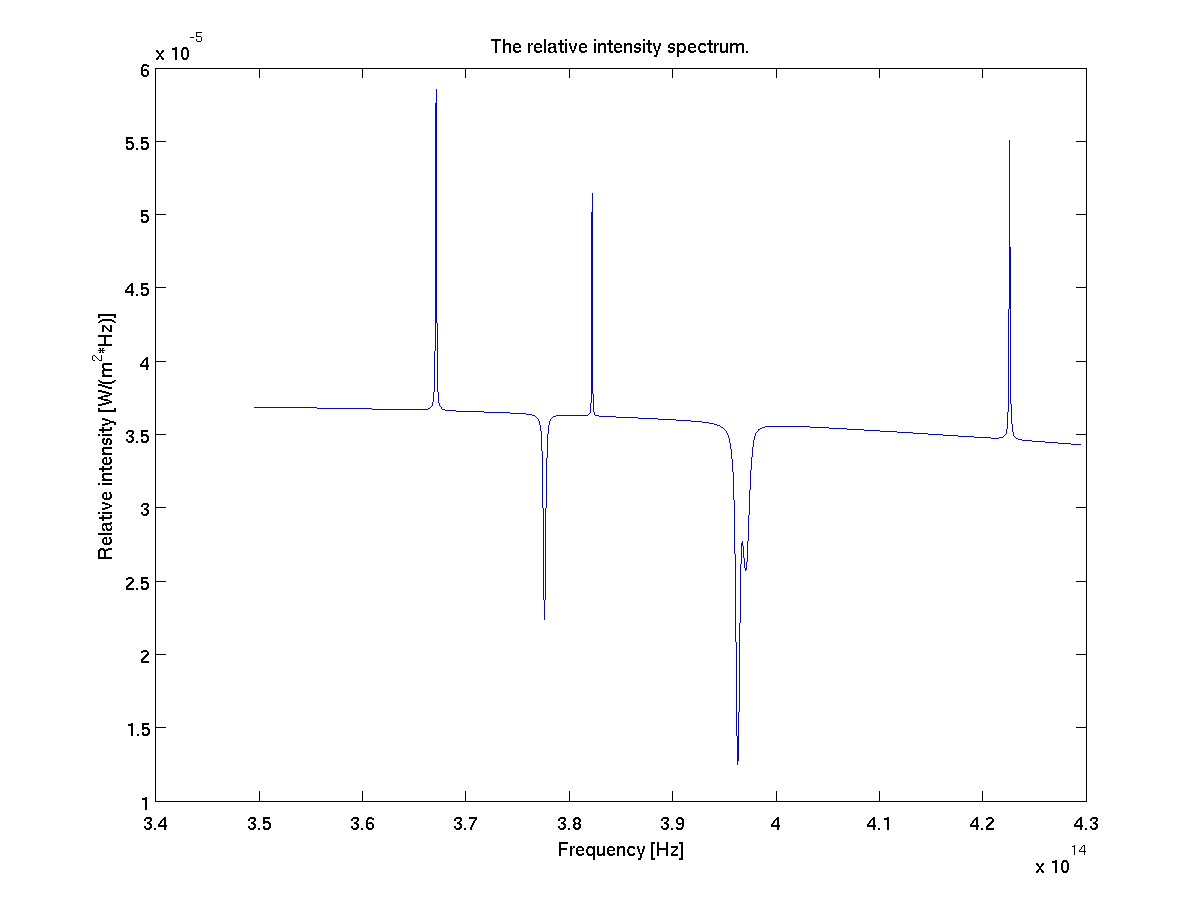
\includegraphics[width=\linewidth]{../img/spectrum_relative.png}
\else
	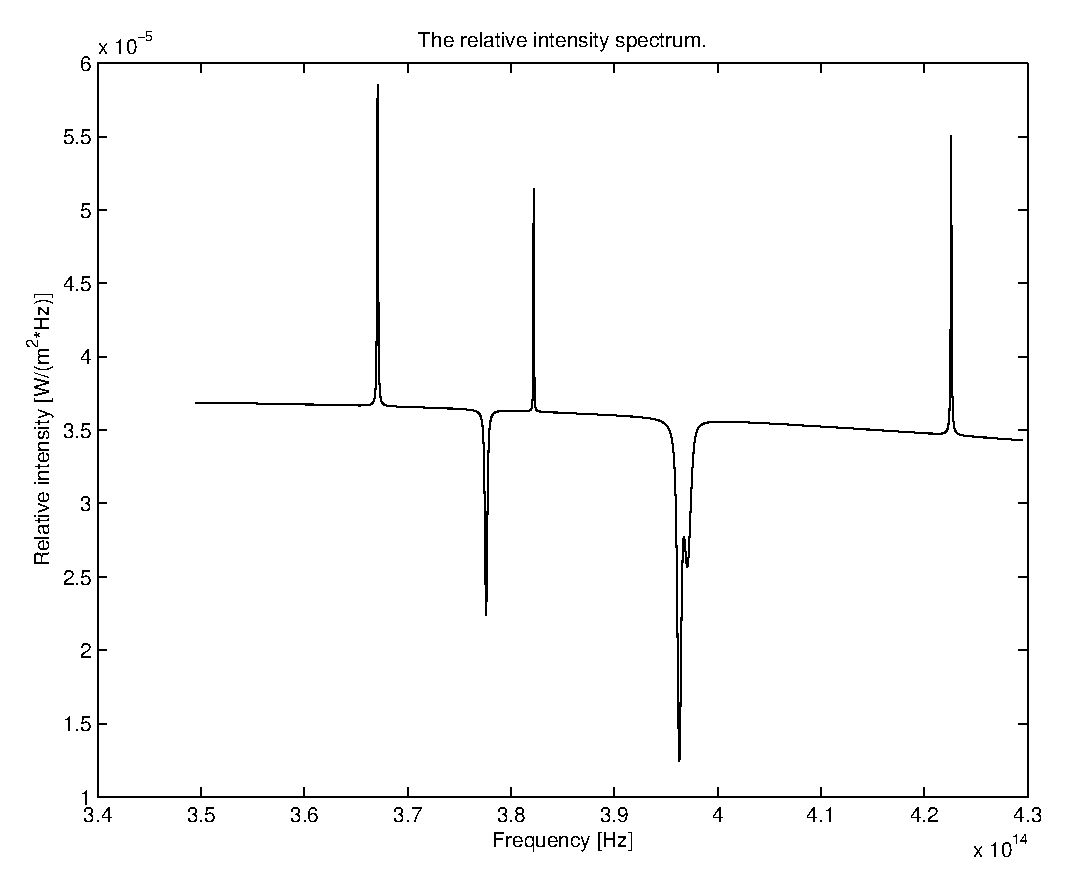
\includegraphics[width=\linewidth]{../img/spectrum_relative.eps}
\fi
\end{center}
\caption{}
\label{fig:rellspec}
\end{figure}

\begin{figure}[hbt]
\begin{center}
\ifpdf
	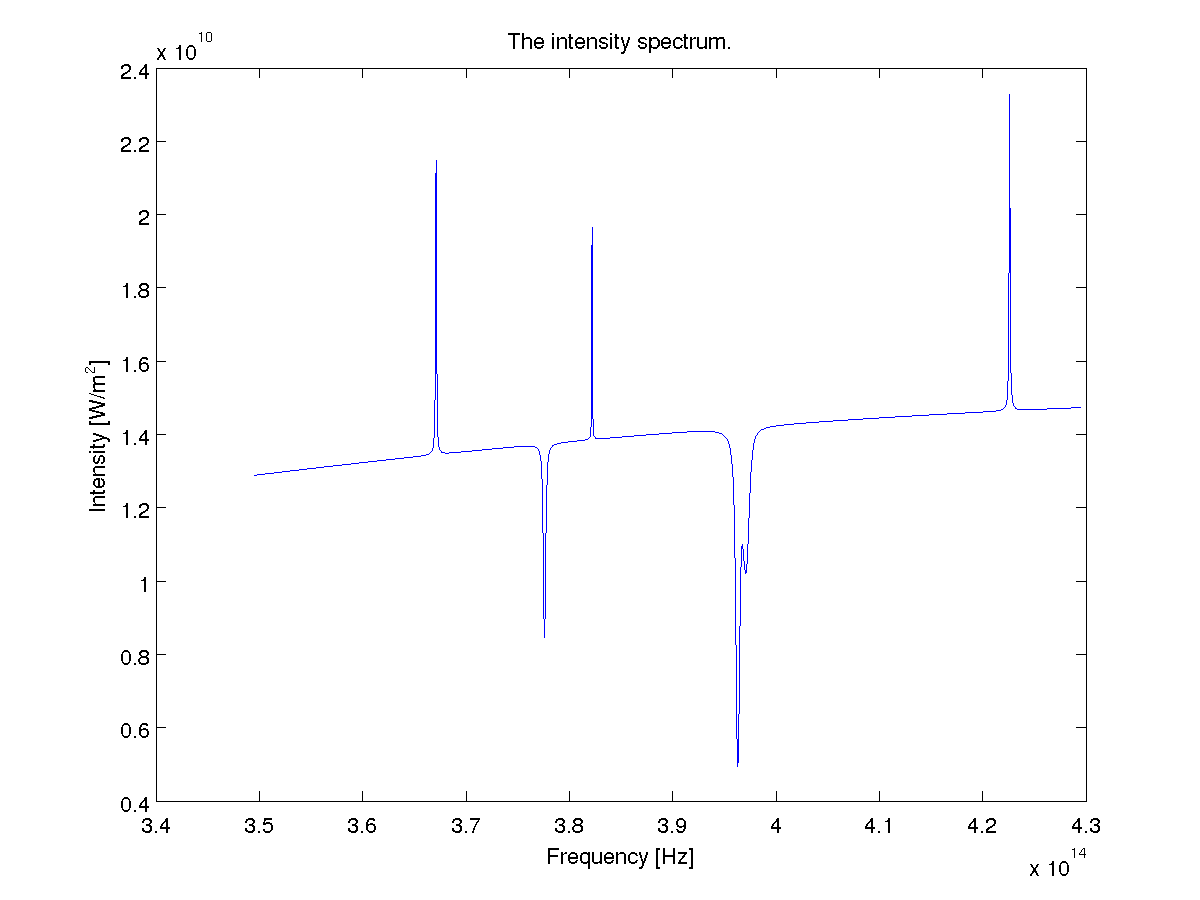
\includegraphics[width=\linewidth]{../img/spectrum.png}
\else
	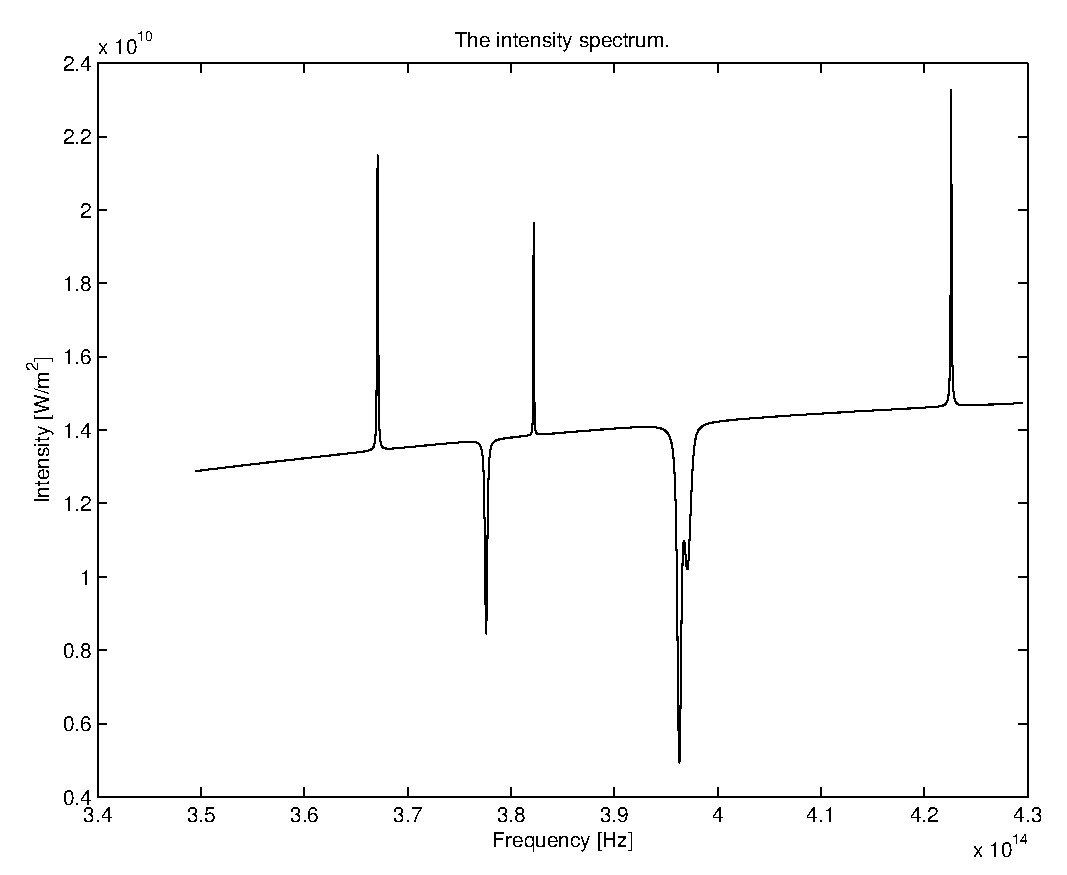
\includegraphics[width=\linewidth]{../img/spectrum.eps}
\fi
\end{center}
\caption{}
\label{fig:spec}
\end{figure}

\begin{figure}[hbt]
\begin{center}
\ifpdf
	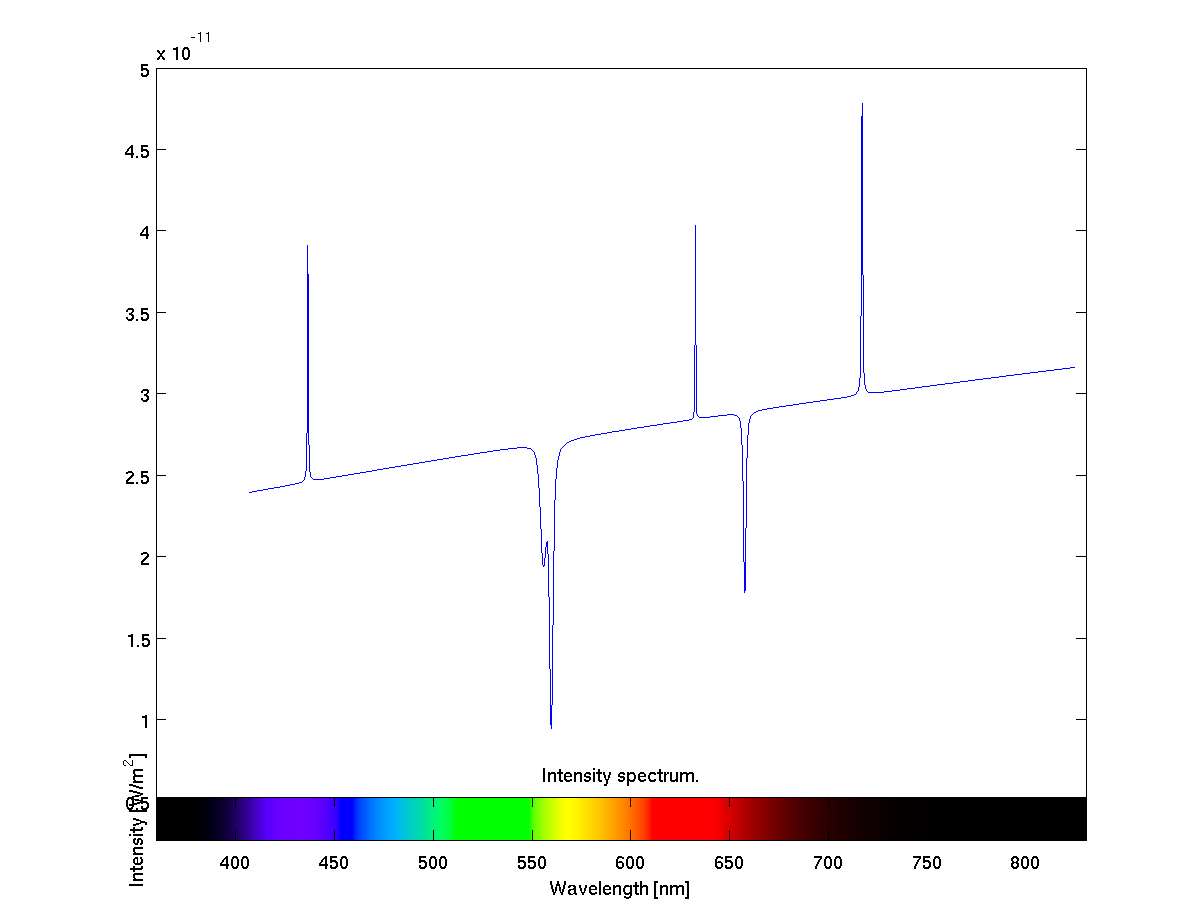
\includegraphics[width=\linewidth]{../img/spectrum_wave.png}
\else
	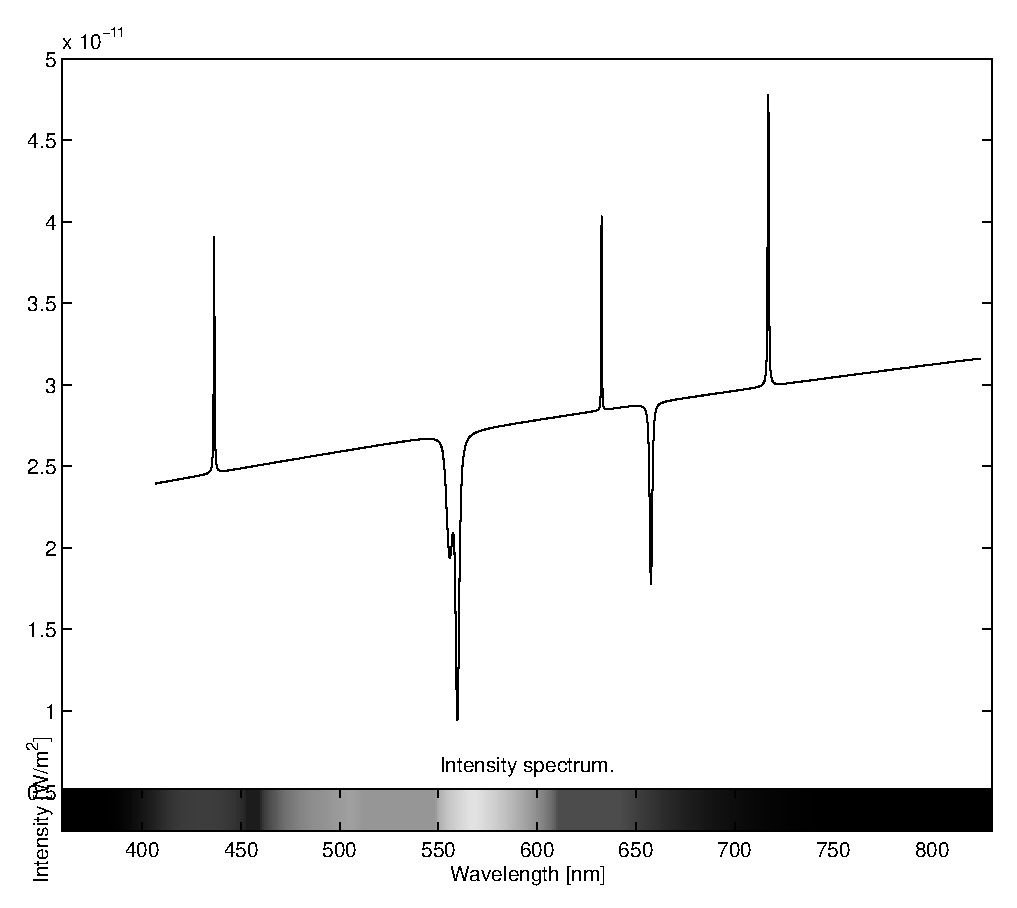
\includegraphics[width=\linewidth]{../img/spectrum_wave.eps}
\fi
\end{center}
\caption{}
\label{fig:specwave}
\end{figure}

\begin{figure}[hbt]
\begin{center}
\ifpdf
	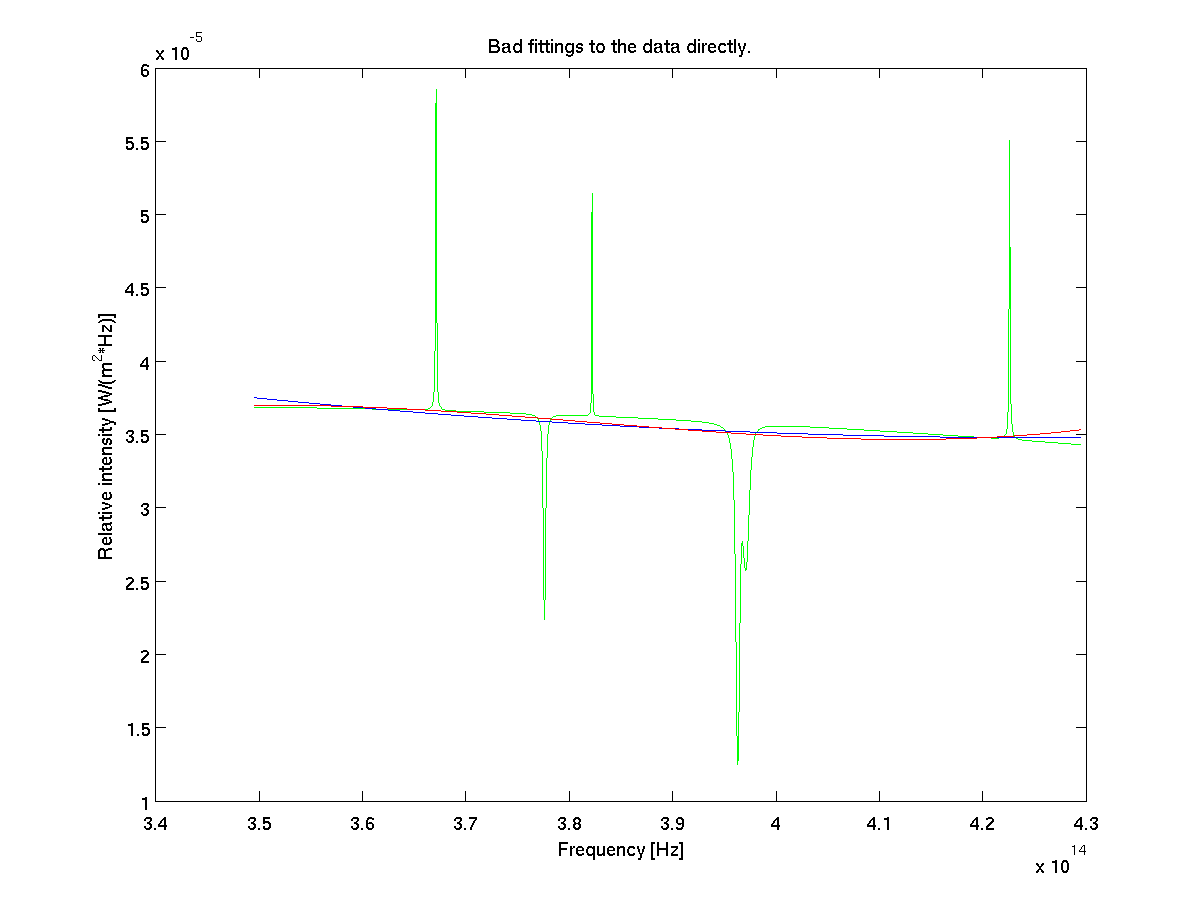
\includegraphics[width=\linewidth]{../img/bad_fits.png}
\else
	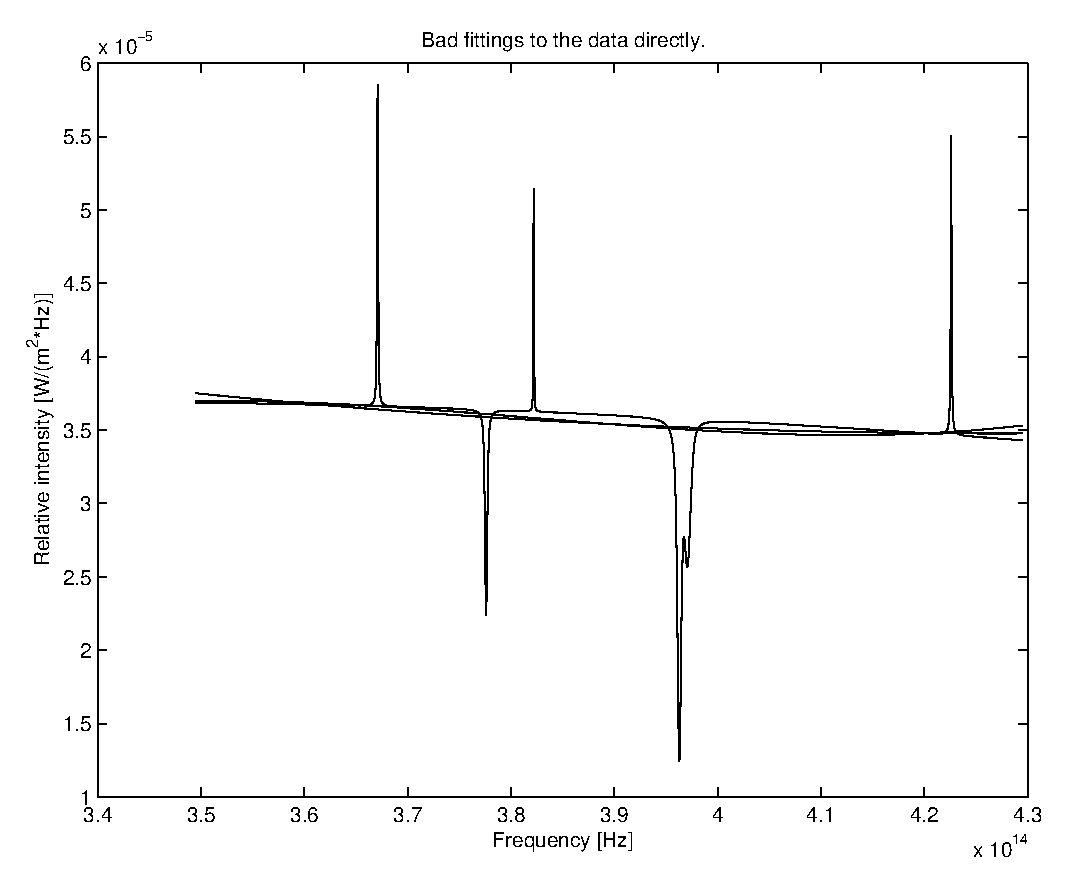
\includegraphics[width=\linewidth]{../img/bad_fits.eps}
\fi
\end{center}
\caption{}
\label{fig:badfit}
\end{figure}

\begin{figure}[hbt]
\begin{center}
\ifpdf
	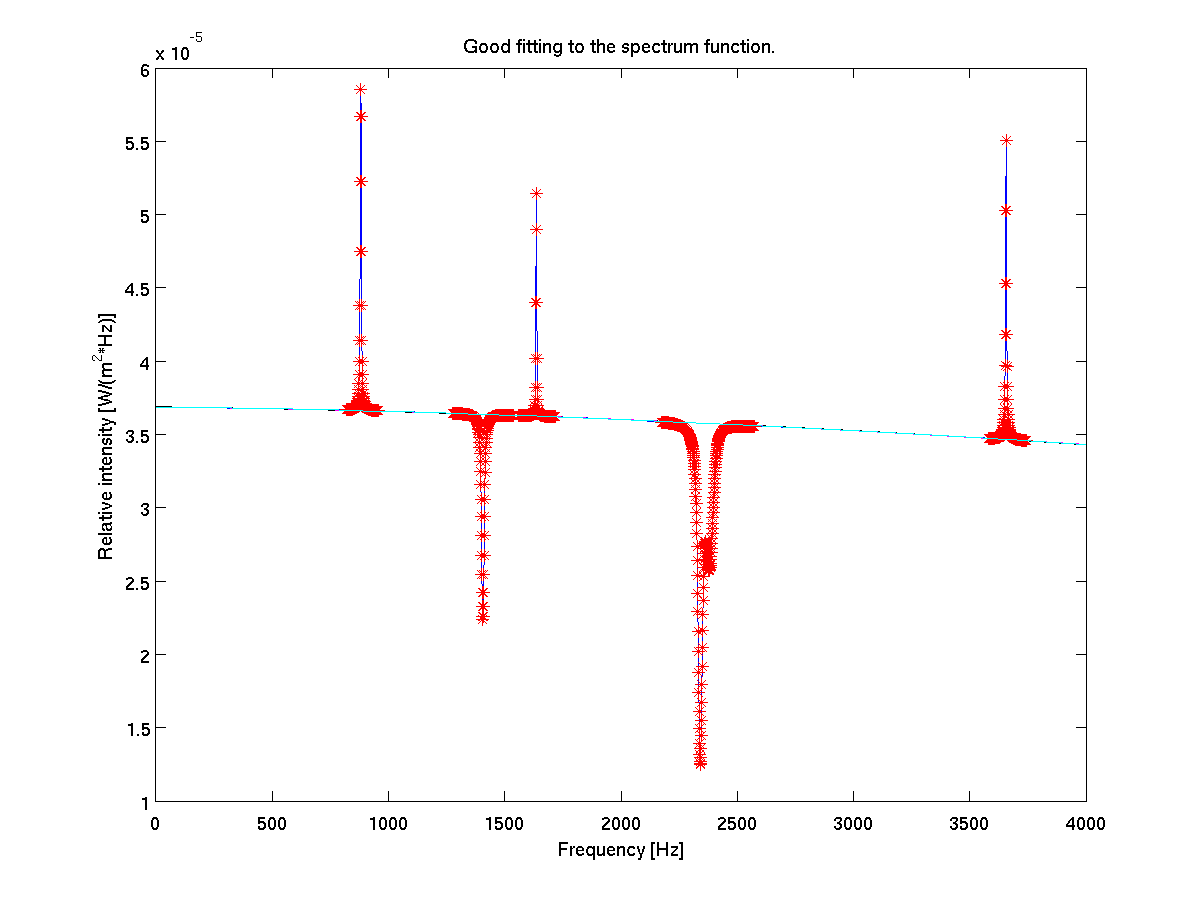
\includegraphics[width=\linewidth]{../img/spectrum_goodfit.png}
\else
	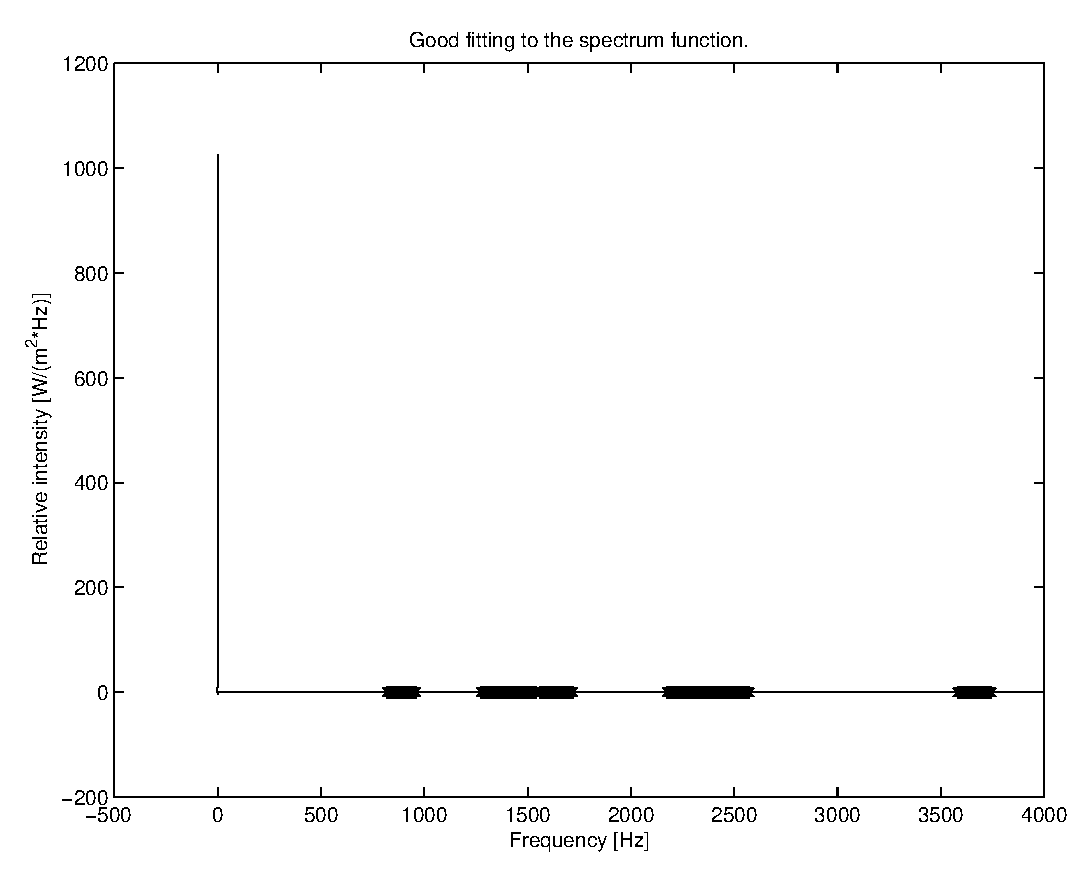
\includegraphics[width=\linewidth]{../img/spectrum_goodfit.eps}
\fi
\end{center}
\caption{}
\label{fig:goodfit}
\end{figure}

\begin{figure}[hbt]
\begin{center}
\ifpdf
	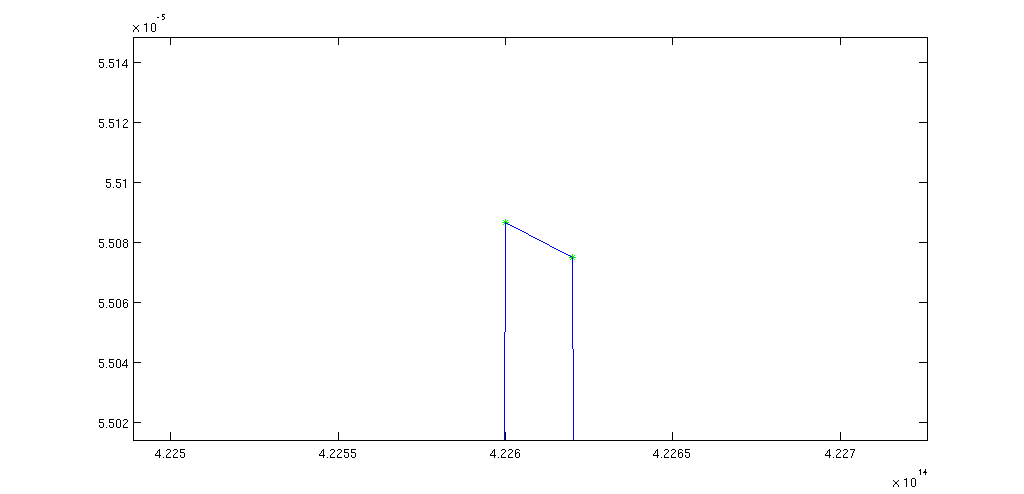
\includegraphics[width=\linewidth]{../img/peak6.png}
\else
	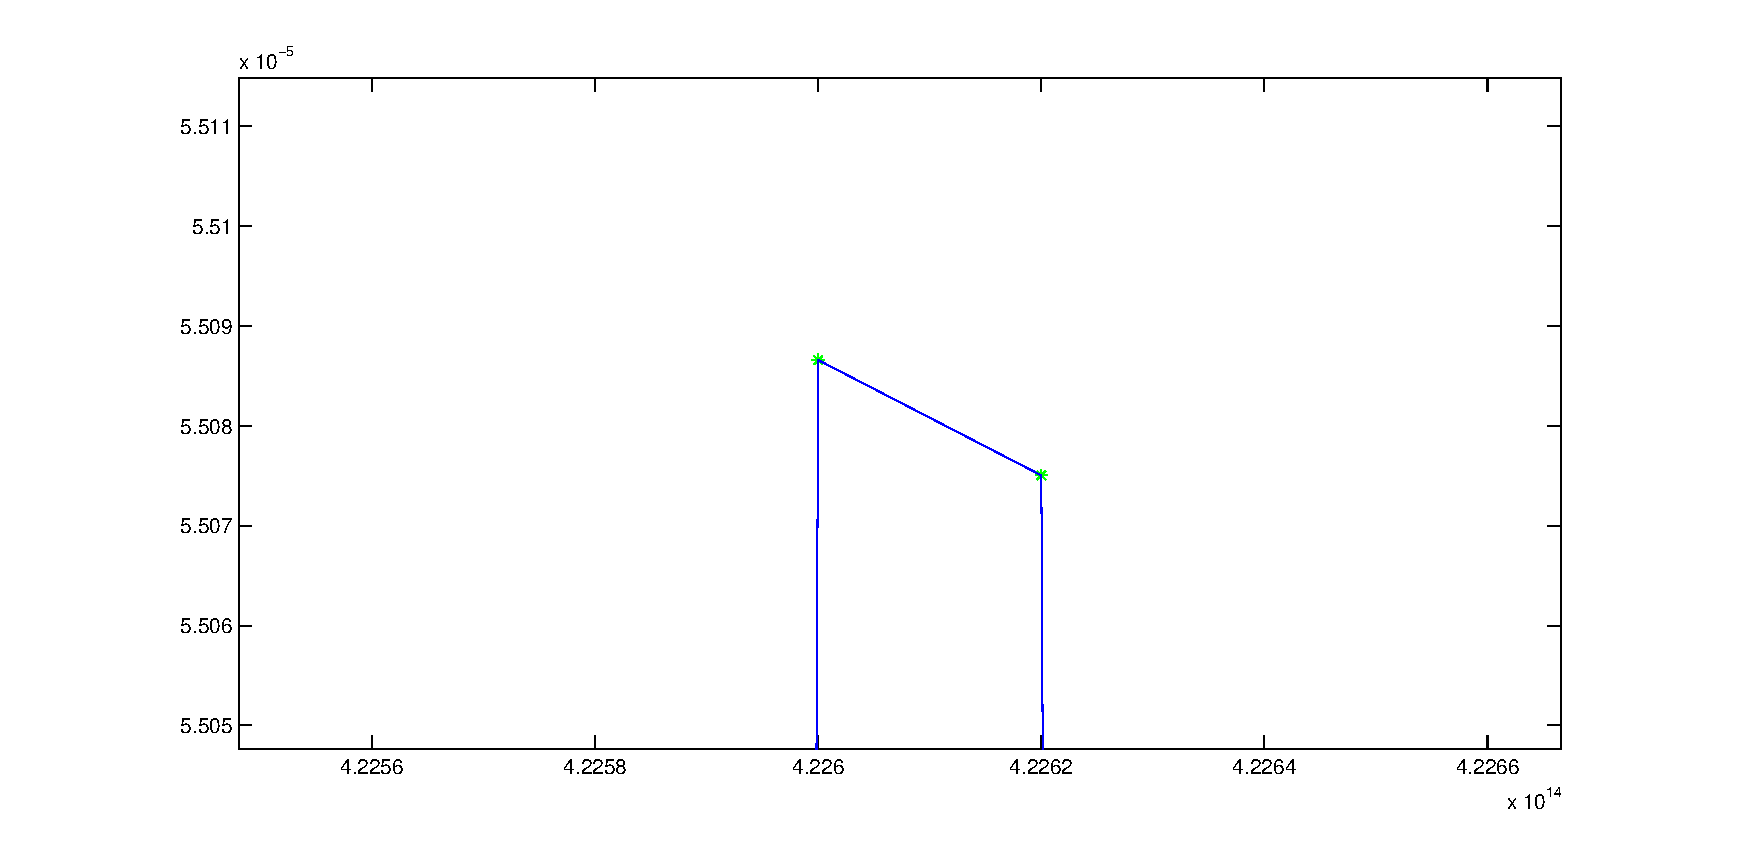
\includegraphics[width=\linewidth]{../img/peak6.eps}
\fi
\end{center}
\caption{The two highest data points for the spectral line.}
\label{fig:peak6}
\end{figure}



\clearpage

\section{Program listings} \label{appendix:programs}
Here the \matlab functions and scripts used to achieve the results above are listed.

\subsection{Scripts}
The following scrips are the drivers for producing the results found in this report.

\lstinputlisting{../src/pr2.m}

\subsection{Functions}
The following functions implements the algorithms and the rest serves as helper functions to these algorithms and the scripts. To distinguish these from other \matlab-functions in the global namespace these reside in a own package called \emph{pr2}.

\lstinputlisting{../src/+pr2/import_data.m}

\end{document}
